\chapter{PET Image Pipeline}
\label{ch:petimages}

This chapter describes a separate experiment on the 599 raw PET acquisitions. Its purpose is to establish whether the images can be processed into reliable quantitative measurements and used by an image model. It does not feed the dementia model, for the reason given in Section~\ref{sec:why_not_images}.

\section{From DICOM series to static volumes}

Each acquisition arrives as a dynamic DICOM series of between 188 and 4,134 files: the same volume repeated over several time frames, from about 20 scanner models. For every scan the stored values were converted to activity concentration, slices were grouped into frames and ordered spatially, and the frames whose mid-point fell inside the tracer's standard static acquisition window (for example 50--70 minutes after injection for florbetapir and PiB, and 90--110 minutes for florbetaben, with five minutes' tolerance) were averaged, each weighted by its duration:
\begin{equation}
V(\mathbf{r}) = \frac{\sum_{k \in \mathcal{W}} d_k\, V_k(\mathbf{r})}{\sum_{k \in \mathcal{W}} d_k},
\end{equation}
where $V_k(\mathbf{r})$ is the activity at voxel $\mathbf{r}$ in frame $k$, $d_k$ the frame duration and $\mathcal{W}$ the set of frames in the window. The result is one static three-dimensional volume per scan. Between two and eight frames, covering 10 to 40 minutes of data, were averaged per scan (Figure~\ref{fig:petqc}). The raw files were only read; all outputs were written to a separate directory.

\section{Spatial registration}

Scans differ in matrix size, voxel spacing and head position, so the same voxel does not correspond to the same anatomical location across scans. No structural MRI was available, so a PET-only registration in two passes was used. In the first pass each scan was aligned to the MNI152 T1 template with a rigid transform (rotation and translation), using mutual information as the similarity measure because PET and T1 images have different contrast. For a fixed image $A$ and a moving image $B$ resampled through the transform $\mathcal{T}$, the mutual information is
\begin{equation}
\text{MI}(A, B \circ \mathcal{T}) = \sum_{a, b} p_{AB}(a, b) \log \frac{p_{AB}(a, b)}{p_A(a)\, p_B(b)},
\end{equation}
where $p_{AB}$ is the joint histogram of intensities (32 bins, Mattes estimator) and $p_A$, $p_B$ its marginals. It is largest when the intensities of one image best predict those of the other, without requiring them to be equal. The transform was optimised by gradient descent over three resolution levels (shrink factors 4, 2, 1), and each scan was smoothed with a Gaussian kernel ($\sigma = 3$~mm) for registration only; the unsmoothed image was resampled for analysis. The aligned scans of each tracer class were averaged to form a study-specific PET template, and in the second pass each scan was aligned to that template with a full affine transform, $\mathcal{T}(\mathbf{r}) = \mathbf{A}\mathbf{r} + \mathbf{t}$, with 12 parameters (nine in $\mathbf{A}$ for rotation, scaling and shear, three in $\mathbf{t}$ for translation). The determinant of $\mathbf{A}$ measures the volume scaling applied; it lay between 0.65 and 1.25 for all scans (Figure~\ref{fig:petqc}). Figure~\ref{fig:petavg} shows the average of the registered scans for each tracer class, which is sharp only if the scans are well aligned. Aligning PET to a PET template is more robust than aligning it to an MRI template.

\begin{figure}[H]
\centering
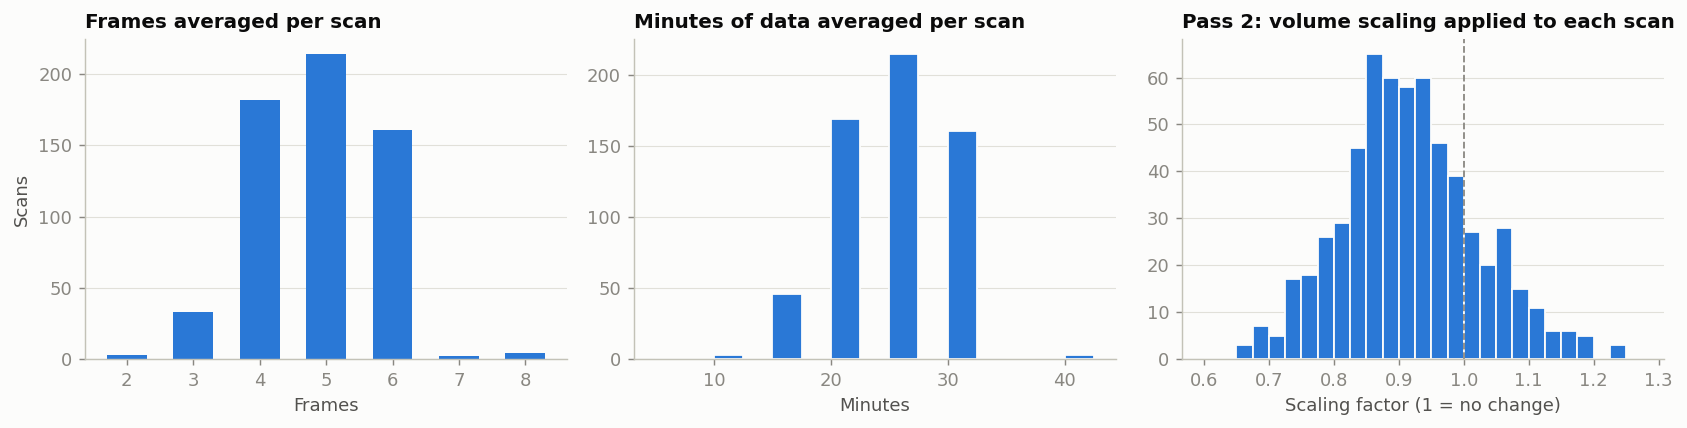
\includegraphics[width=\textwidth]{11_pipeline_qc.png}
\caption{Quality control of the conversion and registration: number of frames and minutes of data averaged per scan, and the volume scaling applied by the affine registration (1 = no change).}
\label{fig:petqc}
\end{figure}

\begin{figure}[H]
\centering
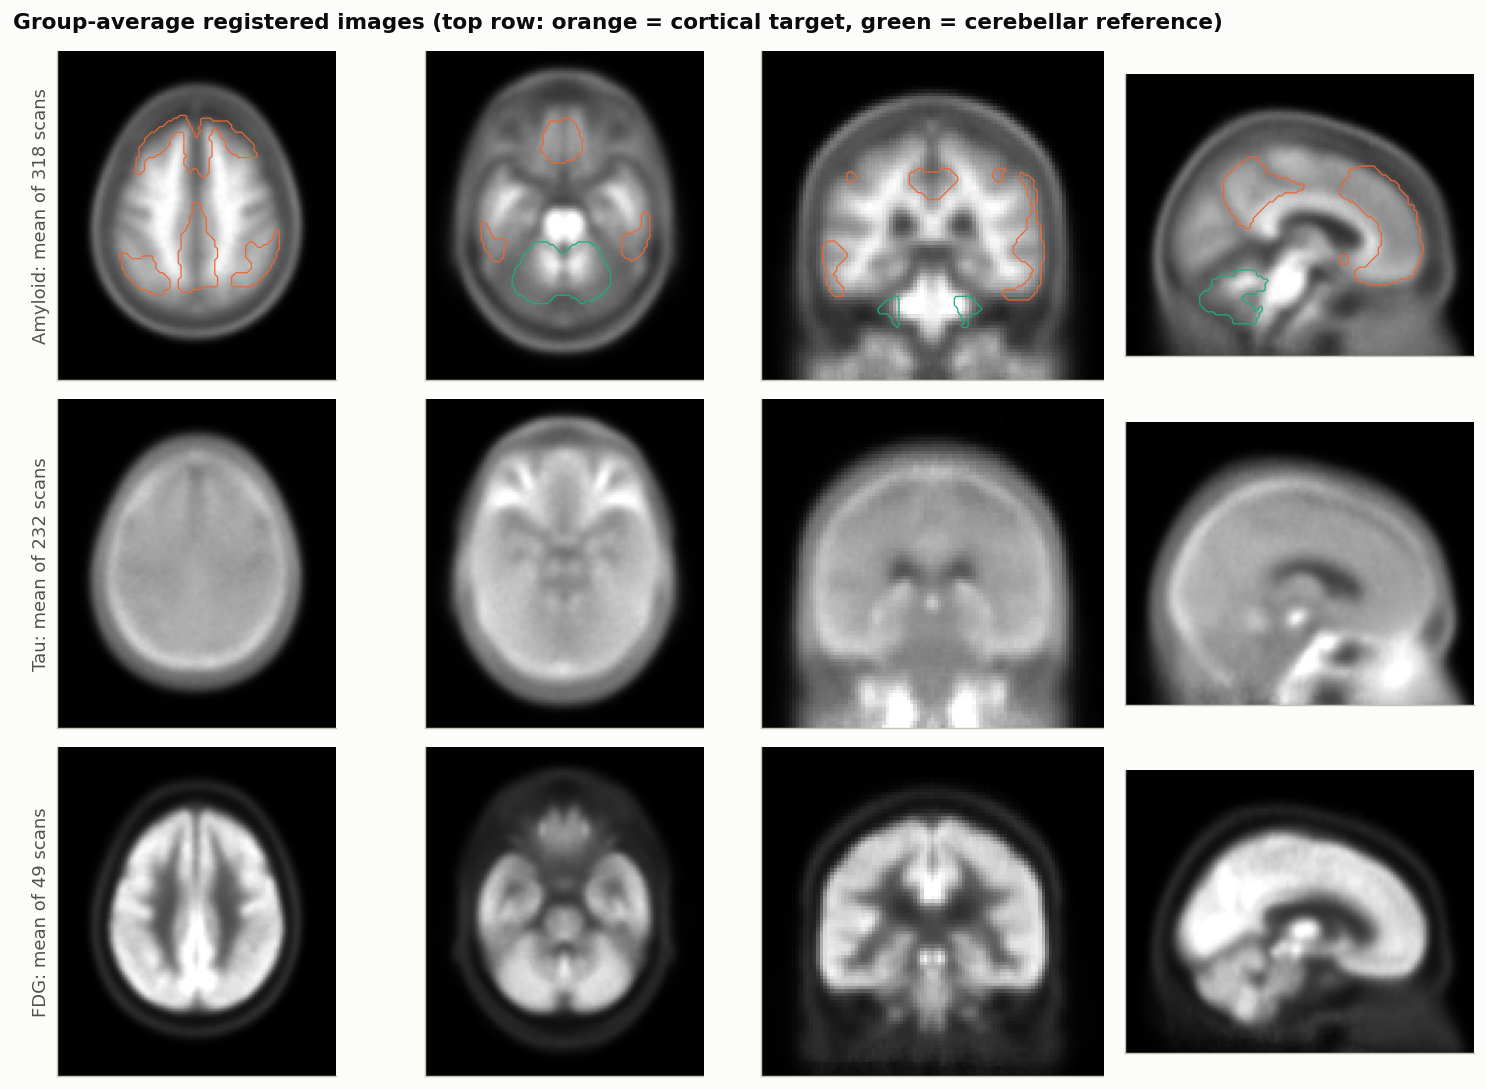
\includegraphics[width=0.92\textwidth]{11_group_average_images.png}
\caption{Average of all registered scans for each tracer class (amyloid, 318 scans; tau, 232; FDG, 49), in axial, coronal and sagittal sections. In the top row the orange outline is the Centiloid cortical target region and the green outline the cerebellar reference region. Only group averages are shown; no individual scan is reproduced.}
\label{fig:petavg}
\end{figure}

\section{Amyloid SUVR from the images}

For each registered amyloid scan, the standardised uptake value ratio was computed as the mean uptake in the cortical target region divided by the mean uptake in the whole cerebellum, using the standard masks of the Centiloid project \cite{klunk2015}:
\begin{equation}
\text{SUVR} = \frac{\frac{1}{|\Omega_{\text{ctx}}|}\sum_{\mathbf{r} \in \Omega_{\text{ctx}}} V(\mathbf{r})}{\frac{1}{|\Omega_{\text{cb}}|}\sum_{\mathbf{r} \in \Omega_{\text{cb}}} V(\mathbf{r})},
\end{equation}
where $\Omega_{\text{ctx}}$ and $\Omega_{\text{cb}}$ are the voxels of the cortical and cerebellar masks. Because the activity scale cancels in the ratio, SUVR does not depend on the injected dose or body weight. NACC's PET core had computed an SUVR for the same scans with a different, MRI-based pipeline in native space. Agreement between the two therefore provides an independent test of the conversion and registration steps. Agreement was summarised by the Pearson and Spearman correlations, the least-squares line $\text{SUVR}_{\text{ours}} = a + b\,\text{SUVR}_{\text{NACC}}$, and the Bland--Altman limits of agreement $\bar{d} \pm 1.96\, s_d$, where $\bar{d}$ and $s_d$ are the mean and standard deviation of the differences $d = \text{SUVR}_{\text{ours}} - \text{SUVR}_{\text{NACC}}$.

\begin{table}[H]
\centering\small
\caption{Agreement between image-derived and NACC amyloid SUVR (318 scans).}
\label{tab:suvr}
\begin{tabular}{@{}lr@{}}
\toprule
Measure & Value \\
\midrule
Pearson correlation & 0.977 \\
Spearman correlation & 0.885 \\
Regression line (ours on NACC) & $-0.16 + 1.10\,x$ \\
Mean difference (ours minus NACC) & $-0.043$ \\
95\% limits of agreement & $-0.18$ to $+0.09$ \\
\bottomrule
\end{tabular}
\end{table}

Agreement was high for every tracer (Pearson $r$ between 0.96 and 0.99 for the four tracers with known identity) and every scanner manufacturer. The lower Spearman correlation reflects the many amyloid-negative scans with similar low values, where small differences change the rank order.

\begin{figure}[H]
\centering
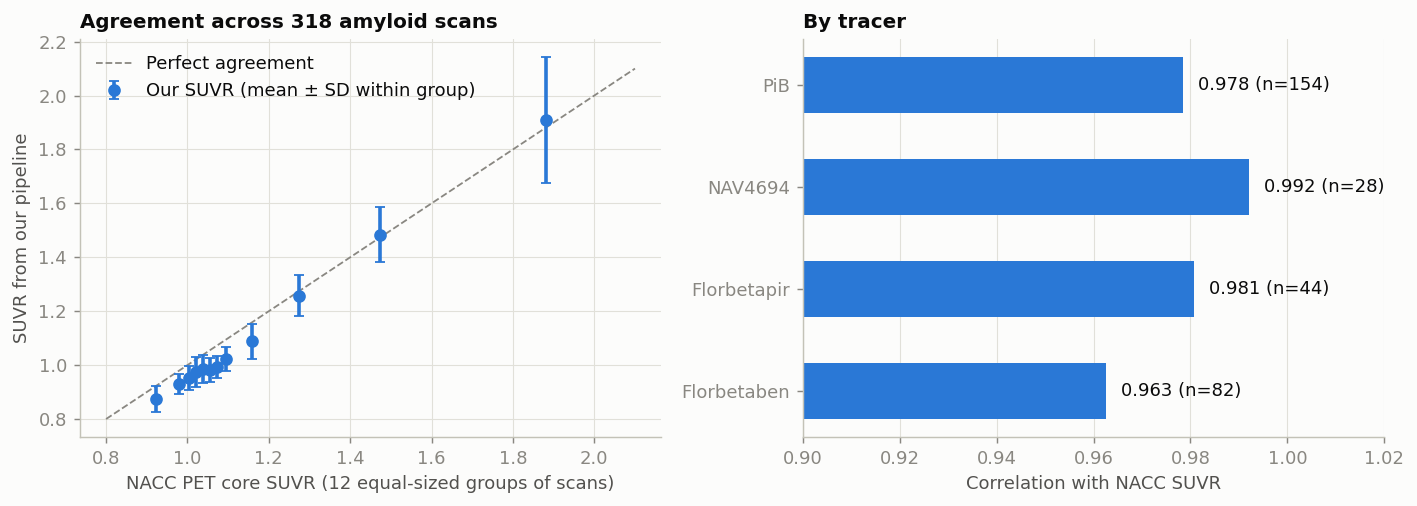
\includegraphics[width=\textwidth]{11_suvr_agreement.png}
\caption{Image-derived amyloid SUVR against the value computed by the NACC PET core for the same scans.}
\label{fig:suvr}
\end{figure}

\section{Amyloid status classification}

Three classifiers of amyloid status were compared on the 292 amyloid scans with a status label from the PET core (84 positive), using five-fold stratified cross-validation so that every scan was predicted by a model that had not seen it: (i) the cortical SUVR alone; (ii) a logistic regression on mean uptake in an $8 \times 8 \times 8$-voxel grid of blocks; and (iii) a small 3D convolutional neural network. The network has four stages of two $3 \times 3 \times 3$ convolutions with instance normalisation and ReLU, each stage halving the resolution, followed by global average pooling, dropout of 0.3 and a linear output, with 494,917 weights in total. Volumes were cropped to the head and resampled to $80 \times 96 \times 80$ voxels. Training used AdamW (learning rate $10^{-3}$, weight decay $10^{-2}$) with a one-cycle schedule, 40 epochs, batches of 8, and augmentation by left--right flips, shifts of up to three voxels and small intensity changes. Because positive scans are the minority, the cross-entropy was weighted,
\begin{equation}
\mathcal{L} = -\frac{1}{n}\sum_i \Big[ w_{+}\, y_i \log \hat{p}_i + (1 - y_i)\log(1 - \hat{p}_i) \Big], \qquad w_{+} = \frac{1 - \bar{y}}{\bar{y}},
\end{equation}
where $\bar{y}$ is the proportion of positive scans in the training folds. The regional logistic model used the mean uptake in each $8 \times 8 \times 8$ block as a feature, with a strong $L_2$ penalty ($C = 0.01$).

\begin{table}[H]
\centering\small
\caption{Amyloid status classification (292 scans, 84 positive, cross-validated).}
\label{tab:cnn}
\begin{tabular}{@{}lr@{}}
\toprule
Method & AUROC \\
\midrule
Cortical SUVR (one number) & 0.982 \\
Regional logistic model & 0.971 \\
3D CNN & 0.960 \\
\bottomrule
\end{tabular}
\end{table}

The single SUVR value performed best (Figure~\ref{fig:cnn}).

\begin{figure}[H]
\centering
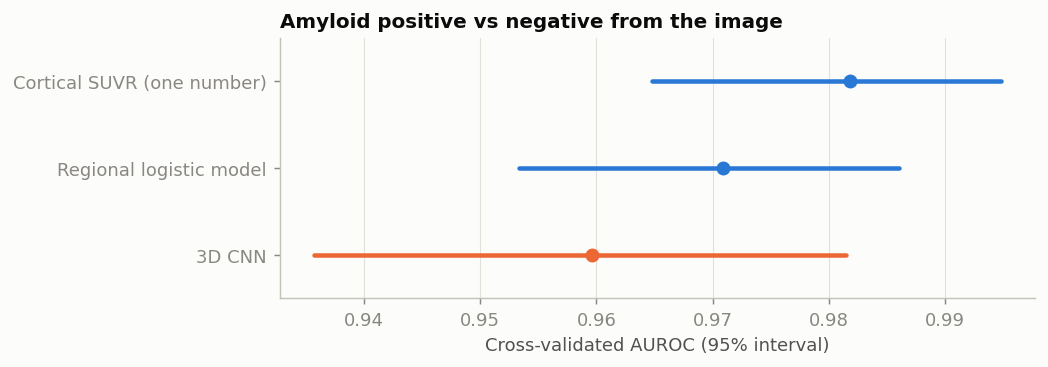
\includegraphics[width=0.85\textwidth]{11_image_models.png}
\caption{Cross-validated AUROC with 95\% bootstrap intervals for the three amyloid-status classifiers.}
\label{fig:cnn}
\end{figure}

 This is expected: the reference label is itself derived by the PET core from a cortical uptake measure, so a scalar SUVR is close to the definition of the label, and a network trained on fewer than 300 scans has little opportunity to improve on it. The experiment shows that the image pipeline supports a working deep-learning model, not that a CNN is preferable for this task.

\section{Grad-CAM}

Gradient-weighted class activation maps \cite{selvaraju2017} were computed for the network and averaged over 72 scans. If $\mathbf{A}^{k}$ is the $k$-th feature map of the last convolutional stage and $s$ the output score, the map is
\begin{equation}
L_{\text{Grad-CAM}} = \operatorname{ReLU}\Big( \sum_k \alpha_k \mathbf{A}^{k} \Big), \qquad
\alpha_k = \frac{1}{Z} \sum_{\mathbf{r}} \frac{\partial s}{\partial A^{k}_{\mathbf{r}}},
\end{equation}
where $Z$ is the number of voxels in the feature map; the map is upsampled to the image size and divided by its maximum. The maps were diffuse: about 96\% of the volume exceeded a quarter of the maximum activation, and only 1.7\% of the most strongly activated voxels lay inside the cortical target region, against 3.8\% expected by chance. The maps therefore do not show that the network attends to the cortical regions where amyloid accumulates, and they are not used as evidence of what the model has learned. Figure~\ref{fig:gradcam} shows the group-average images of amyloid-negative and amyloid-positive scans together with the mean Grad-CAM map: the positive scans show the expected higher cortical uptake, whereas the map is highest at the lower edge of the brain rather than in the cortical target region.

\begin{figure}[H]
\centering
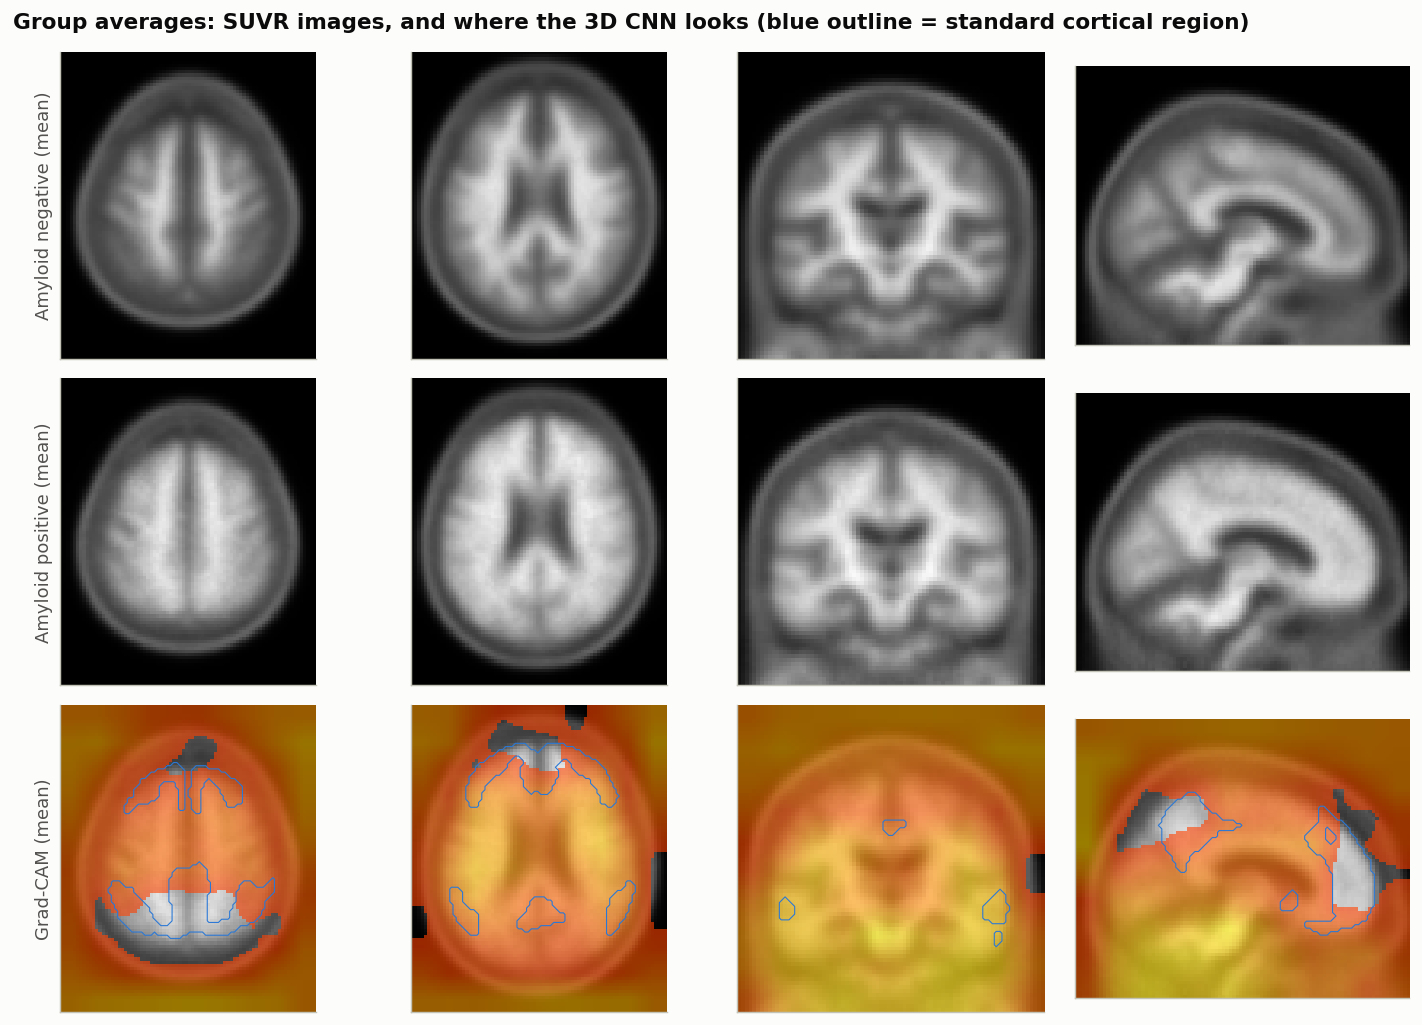
\includegraphics[width=0.92\textwidth]{11_gradcam_mean.png}
\caption{Group-average SUVR images of amyloid-negative and amyloid-positive scans (top two rows) and the mean Grad-CAM map of the 3D CNN (bottom row), in four sections. The blue outline marks the standard cortical target region.}
\label{fig:gradcam}
\end{figure}

\section{Why images are not used to predict dementia}
\label{sec:why_not_images}

Of the 446 participants with an image, about 86\% were cognitively normal at the time of the scan, follow-up after the scan is about two years, and only five later received a dementia diagnosis. No model can learn a reliable pattern from five events, so dementia prediction from images was not attempted. The quantitative PET information that is available for thousands of participants is used instead, through the late-fusion model described in Chapter~\ref{ch:method}.

Two further limitations apply. Registration without an MRI is less precise than the MRI-based pipelines used by PET cores. Tau images were converted and registered but not quantified, because a standard tau target mask comparable to the Centiloid masks was not available.
